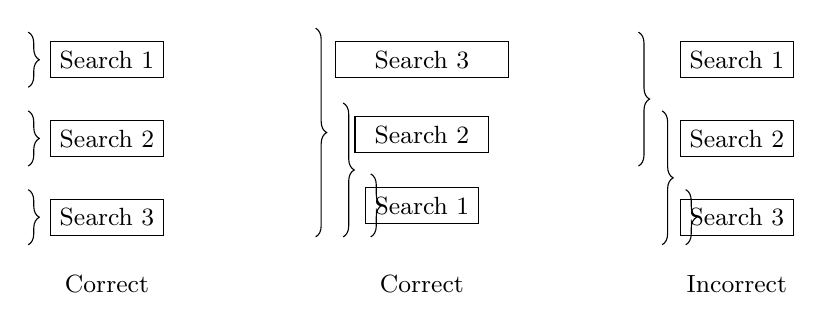
\begin{tikzpicture}[font=\small,
  block/.style={draw,minimum width=1.4cm,minimum height=0.45cm,align=center},
  brace/.style={decorate,decoration={brace,amplitude=4pt}}]
  % Independent searches
  \node[block] (a1) at (0,1.5) {Search 1};
  \node[block] (a2) at (0,0.5) {Search 2};
  \node[block] (a3) at (0,-0.5) {Search 3};
  \draw[brace] (-1.0,1.85) -- (-1.0,1.15);
  \draw[brace] (-1.0,0.85) -- (-1.0,0.15);
  \draw[brace] (-1.0,-0.15) -- (-1.0,-0.85);
  \node at (0,-1.35) {Correct};

  % Nested searches
  \node[block,minimum width=2.2cm] (b3) at (4.0,1.5) {Search 3};
  \node[block,minimum width=1.7cm] (b2) at (4.0,0.55) {Search 2};
  \node[block,minimum width=1.2cm] (b1) at (4.0,-0.35) {Search 1};
  \draw[brace] (2.65,1.9) -- (2.65,-0.75);
  \draw[brace] (3.0,0.95) -- (3.0,-0.75);
  \draw[brace] (3.35,0.05) -- (3.35,-0.75);
  \node at (4.0,-1.35) {Correct};

  % Intersecting searches
  \node[block] (c1) at (8.0,1.5) {Search 1};
  \node[block] (c2) at (8.0,0.5) {Search 2};
  \node[block] (c3) at (8.0,-0.5) {Search 3};
  \draw[brace] (6.75,1.85) -- (6.75,0.15);
  \draw[brace] (7.05,0.85) -- (7.05,-0.85);
  \draw[brace] (7.35,-0.15) -- (7.35,-0.85);
  \node at (8.0,-1.35) {Incorrect};
\end{tikzpicture}
